Lex et yacc sont des outils similaire : ce sont tous les deux gérateur d’analyseur syntaxique.

Leur fonctionnement est très similaire dans le sens où il permettent d'associer des actions lorsque qu'un mot du texte en entrée est reconnu.

Cependant, le fonctionnement de yacc est légèrement plus puissant. En effet, il permet de fonctionner avec une grammaire.

Le code yacc est divisé en 3 partie que nous allons voir rapidement.

\subsection{première partie}
cette première partie commence par \%\{ et finie par \%\}. Elle permet de définir tous les besoins du code c/c++. C'est à dire la déclaration des variables, des constantes, des fonctions,etc...

\subsection{deuxième partie}
Cette partie contient l'ensemble de la grammaire et des actions qui lui sont associé. C'est dans cette partie que yacc se distingue de Lex.
En effet, là où Lex utilise des définitions régulières et un ensemble de règles, Yacc se contente d'associer à chaque règle d'une grammaire une ou des actions c++.

A l'exécution, cette différence s'exprime par le fait que les règles de Lex sont fixes. Lex va essayer de trouver le mot le plus long qui permet de matcher à une règle. C'est à dire qu'il y à un match pour une seule règle. Une fois le mot trouvé, Lex "oublie" totalement la règle utilisé et passe à la recherche du mot suivant.
Yacc lui permet de remonter les règles et donc d'effectuer plusieurs actions à différents moments sur une même chaîne de caractère. C'est à dire qu'il va se souvenir des règles qu'il traverse.
Ce fonctionnement ressemble fortement à ce que nous avons fais dans le code : parcourir l'arbre de notre grammaire et effectuer des actions en fonction du noeud où nous sommes. Yacc fonctionne exactement pareil.

cette grammaire se définie de la manière suivante : \newline

\begin{tabular}{|c|}
    \hline
        NON\_TERMINAL: expression \\
    \hline
\end{tabular}
\newline

En premier, le non-terminal suivie de deux points. Puis une expression pouvant contenir des non-terminaux, des terminaux ou des symboles spéciaux tel que | pour la règle "ou" des grammaire, etc...

\subsection{troisième partie}
Cette partie est la déclaration des fonctions c++ de la première partie et de la déclaration de la fonction principale du programme.

\subsection{exemple de code Yacc}
Vous pourrez trouvez un exemple de code Yacc dans le dossier de ce rapport.
Ce code yacc permet de récupérer des opérations d'additions ou de multiplication entre des entiers (deux,trois, quatre, ...) et d'afficher le resultat dans la sortie standard. Le code est contenue dans le fichier essai\_yacc.yxx.
Celui-ci peut être compilé avec les commande :\newline

\begin{tabular}{|c|}
    \hline
        \$ yacc essai\_yacc.yxx \\
        cela générera un fichier y.tab.c mais qui devra être compilé \\
         avec un compilateur c++ (dû à l'utilisation d'iostream et des cout,cin)\\
    \hline
        \$ g++ y.tab.c \\
        (générera l'exécutable qui peut être lancé avec la commande \$ ./a.out) \\
    \hline
\end{tabular}
\newline

Le résultat du code est le suivant, de la forme " $-->$ resultat\_operation ":
\newline

\begin{figure}[h]
    \centerline{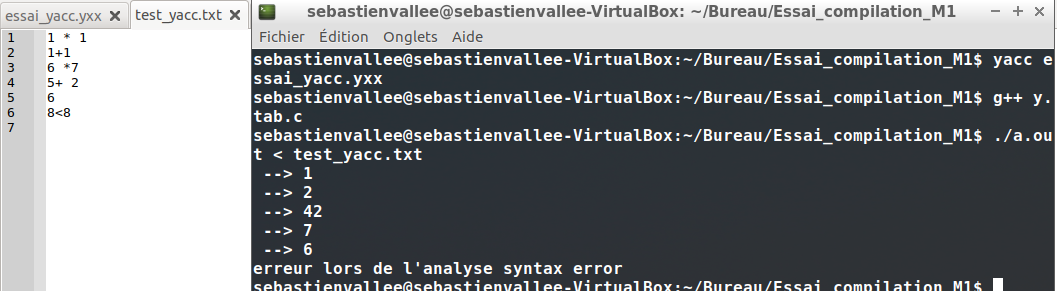
\includegraphics[scale=0.7]{data/yacc}}
    \caption{resultat du code yacc}
    \label{fig:yacc}
\end{figure}

Sur la figure \href{fig:yacc}{2}, on peut voir que le programme s'arrête sur une erreur : la dernière ligne "8 $<$ 8" ne respecte aucune règle donc le mot (tout le fichier) est faux et le programme s'arrête.

\newpage